\documentclass{article}
\usepackage{graphicx} % Required for inserting images
\usepackage[margin=1in]{geometry}
\usepackage{amsmath}
\usepackage{amsthm}
\usepackage{amssymb}
\usepackage{amsfonts}
\usepackage{verbatim}
\usepackage{xcolor}

\title{Homework 2: Report}
\author{Dante Buhl}
\date{Jan $20^{th}$ 2024}

\begin{document}

\newcommand{\bs}[1]{\boldsymbol{#1}}
\newcommand{\bmp}[1]{\begin{minipage}{#1\textwidth}}
\newcommand{\emp}{\end{minipage}}
\newcommand{\R}{\mathbb{R}}
\newcommand{\C}{\mathbb{C}}
\newcommand{\N}{\mathcal{N}}
\newcommand{\I}{\mathrm{I}}
\newcommand{\K}{\bs{\mathrm{K}}}
\newcommand{\m}{\bs{\mu}_*}
\newcommand{\s}{\bs{\Sigma}_*}
\newcommand{\dt}{\Delta t}
\newcommand{\tr}[1]{\text{Tr}(#1)}
\newcommand{\Tr}[1]{\text{Tr}(#1)}

\maketitle


\begin{enumerate}

\item %start of problem 1
Let $A \in C^{m\times m}$ be both upper-triangular and unitary. Show that A is a
diagonal matrix. Does the same hold if $A \in C^{m\times m}$ is both lower-triangular
and unitary?

\begin{proof}

\textbf{ (Upper Triangular, by Induction)}

Assume matrix $A \in \C^{m \times m}$ is unitary and is upper triangular such that,

\[ 
    A^*A = \mathrm{I}_m = AA^*
\]

\[
    A = \left[\begin{array}{c c c c}
        a_{11} & a_{12} & \cdots & a_{1m} \\
        0 & a_{22} & \cdots & a_{2m} \\
        \vdots & \vdots & \ddots & \vdots \\
        0 & 0 & \cdots  & a_{mm}
        \end{array}\right]
\] 

Where $A^*$ is the complex transpose matrix of $A$. We have then that $A^*$ is of the form, 

\[
    A^* = \left[\begin{array}{c c c c}
        \overline{a_{11}} & 0 & \cdots & 0 \\
        \overline{a_{12}} & \overline{a_{22}} & \cdots & 0 \\
        \vdots & \vdots & \ddots & \vdots \\
        \overline{a_{1m}} & \overline{a_{2m}} & \cdots  & \overline{a_{mm}}
        \end{array}\right]
\] 

Then the product of matrix multiplication of $A^*$ and $A$ is then defined as $B$, (i.e. $B = A^*A$), and because A is a Unitary matrix, is equal to $\mathrm{I}$. 

\textbf{(Base Case)}: 

Now assume that the elements above the diagonal in $A$ are non-zerp. Next examine the $(1, 1)$ and $(2, 1)$ cells of the matrix product, $B$. By the operation of Matrix multiplication we should have, 
\[
    B(2, 1) = a_{11} \cdot \overline{a_{12}} = \mathrm{I}_m(2, 1) = 0
\]
\[
    B(1, 1) = a_{11} \cdot \overline{a_{11}} = \mathrm{I}_m(1, 1) = 1
\]
From this, we know that $a_{11} \neq 0$ and $\overline{a_{11}} \neq 0$. But we have that the product of $a_{11} \cdot \overline{a_{12}} = 0$. Since we have that  $a_{11} \neq 0$, we must therefore have that $\overline{a_{12}} = 0$ and by the definition of a complex conjugate, $a_{12} = 0$. 

\textbf{(Inductive Step)}

We need to show that for a integer $k \le m-1$ all of the columns of matrix $A$, $\vec{C}_i$, up to $\vec{C}_k$ is of the form, 
\[
    \vec{C}_i = \left[\begin{array}{c}
                0 \\
                \vdots \\
                a_{ii} \\
                \vdots \\
                0
                \end{array}\right]
\]
then $\vec{C}_{k+1}$ is also of the same form. We have that in the matrix product between $A^*$ and $A$, $B$, then the i-th row of $B$ is defined as the inner produt between the i-th row of $A^*$, $\vec{r}_i^*$ and the j-th column of $A$, $\vec{c}_j$.  
\[
    B(i, :) = [(\vec{r}_i^*, \vec{c}_1), (\vec{r}_2^*, \vec{c}_2), \cdots, (\vec{r}_i^*, \vec{c}_j)] = \mathrm{I}_m(i, :) = [0, \cdots, 1, \cdots, 0]
\]

Look at the $(k+1)$-th row of B. We have from the given form of the columns, $\{\vec{c}_1, \cdots, \vec{c}_k\}$, 
\[
    (\vec{r}_{k+1}^*, \vec{c}_j) = \overline{a_{j(k+1)}}\cdot a_{jj} = \left\{\begin{array}{c c c}
                                                                0 & \text{if, } & j \neq k+1\\
                                                                1 & \text{if, } & j = k+1
                                                            \end{array}\right\}, i, j < k+1
\]
We also have that each $a_{ii} \neq 0$. Thereby, for all $j < k+1$, 
\[\overline{a_{j(k+1)}} = 0 \implies a_{j(k+1)} = 0\]We now write the column, $\vec{c}_{k+1}$. 
\[  
    \vec{c}_{k+1} = \left[\begin{array}{c}
                    0 \\
                    \vdots \\
                    a_{(k+1)(k+1)} \\
                    \vdots \\
                    0
                    \end{array}\right]
\]
Therefore, we have that $\vec{c}_{k+1}$ is of the same form as $\vec{c}_{i}, i \le k$. By induction, each column of $A$ is of this form. Therefore, $A$ is a diagonal matrix!


\end{proof}

\begin{proof}

\textbf{(Lower Triangular, by case of Upper Triangular)}

Assume as before,  $A \in \C^{m \times m}$ is unitary and is lower triangular such that,

\[ 
    A^*A = \mathrm{I}_m = AA^*
\]

\[
    A = \left[\begin{array}{c c c c}
        a_{11} & 0 & \cdots & 0 \\
        a_{21} & a_{22} & \cdots & 0 \\
        \vdots & \vdots & \ddots & \vdots \\
        a_{m1} & a_{m2} & \cdots  & a_{mm}
        \end{array}\right]
\] 

Where $A^*$ is the complex transpose matrix of $A$. We have then that $A^*$ is of the form, 

\[
    A^* = \left[\begin{array}{c c c c}
        \overline{a_{11}} & \overline{a_{21}} & \cdots & \overline{a_{m1}} \\
        0 & \overline{a_{22}} & \cdots & \overline{a_{m2}} \\
        \vdots & \vdots & \ddots & \vdots \\
        0 & 0 & \cdots  & \overline{a_{mm}}
        \end{array}\right]
\] 

We then define the matrix $C = A^*$, $C^* = A$. Notice that C is an upper triangular, unitary matrix. By the previous proof, $C$ is a diagonal matrix. Notice all of its ``off-diagonal'' elements are zero. As a consequnce, all (i, j)-elements of $C$ which are zero imply that (j, i)-elements of $C^*$ are zero. Therefore, $C^* = A$ is a diagonal matrix.


\end{proof}%end of problem 1

\item %start of problem 2
Prove the following in each problem.
\begin{enumerate}

    \item
    Let $A \in \C^{m \times m}$ be invertible and $\lambda \neq 0$ is an eigenvalue of $A$. Showthat $\lambda^{-1}$ is an eigenvalue of $A^{-1}$.

    \begin{proof}

    Take any $A \in \C^{m\times m}$ to be invertible. Then we have inverse, $A^{-1}$ exists such that, 
    \[
        AA^{-1} = \mathrm{I}_m = A^{-1}A
    \]
    We also have by the fact that $\lambda \neq 0$ is an eigenvalue of $A$ that, 
    \[
        \text{det}(A - \lambda\mathrm{I}_m) = 0
    \]
    We can substitute for $\I_m$.
    \[
        \text{det}(A - \lambda\I_m) = \text{det}(A - \lambda(A^{-1}A)) =     \text{det}(A)\text{det}(\I_m - \lambda A^{-1}) = 0 
    \]
    \[
        \text{det}(I_m - \lambda A^{-1}) = -\text{det}(A^{-1} - \frac{1}{\lambda}\I_m) = 0
    \]
    \[
        \text{det}(A^{-1} - \frac{1}{\lambda}\I_m) = 0
    \]
    Therefore, $\lambda^{-1}$ is an eigenvalue of $A^{-1}$.
    
    \end{proof}


    \item 
    Let $A, B \in \C^{m\times m}$. Show that $AB$ and $BA$ have the same eigenvalues.
    
    \begin{proof}
    
    Let $A, B$ be square matrices as shown above. Now look at some eigenvalue of the   matrix product $AB$, $\lambda$. We have by definition of an eigenvalue the following equality.
    \[
        AB\vec{v} = \lambda\vec{v}
    \]
    Now we multiply both vectors by the matrix $B$.
    \[
        B(AB\vec{v}) = B(\lambda\vec{v})
    \]
    \[
       (BA)(B\vec{v}) = \lambda(B\vec{v})  
    \]
    \[
        BA\vec{w} = \lambda\vec{w}
    \]
    Therefore $\lambda$ is also an eigenvalue of the matrix product $BA$. Since our choice of $\lambda$ was arbitrary, we have that all eigenvalues of $AB$ are eigenvalues of $BA$. 
    \end{proof}


    \item 
    Let $A \in \R^{m \times m}$. Show that $A$ and $A^*$ have the same eigenvalues. (Hint 1: Use det($M$) = det($M^T$) for any square matrix $M \in \R^{m\times m}$ in connection to the definition of characteristic polynomials. Hint 2: When a real-valued matrix $A$ has a complex eigenvalue $\lambda$, then $\overline{\lambda}$ is also an eigenvalue of $A$.)

\begin{proof}
    
First look at an an arbitrary eigenvalue, $\lambda$, of $A$.
\[
    \text{det}(A - \lambda\I) = 0
\]
We examine the determinant of a conjugate transpose. Since determinant is the sum/difference of the products along the diagonals, we have that the determinant of the conjugate tranpose is equivalent to the complex conjugate of the determinant of the tranpose. 
\[
    \det(A^*) = \overline{\det(A^T)} = \overline{\det(A)}
\]
We then look at the definition of the characteristic polynomial. 
\[
    \det(A-\lambda\I) = 0 \implies \overline{\det(A - \lambda\I)} = 0 = \det[(A - \lambda\I)^*]  = \det(A^* - \overline{\lambda}\I)
\]
        We have then that the complex conjugate of all eigenvalues of $A$ are eigenvalues of $A^*$. We also notice that since $A$ and $A^*$ are real, that the characteristic polynomials are also real. Thus if we are to have a complex number as a root of a real polynomial, the complex conjugate must also be a root. Thereby, all complex $\lambda$ and their conjugates $\overline{\lambda}$ are roots of both $A$ and $A^*$. Moreover, if $\lambda$ is not complex it is automatically a root of both $A$ and $A^*$. 
        \end{proof}
    \end{enumerate} %end of problem 2

\item   %start of problem 3
Let $A \in \C^{m \times m}$ be hermitian. Suppose that for nonzero eigenvectors of $A$, there exist corresponding eigenvalues $\lambda$ satisfying $Ax = \lambda x$.

\begin{enumerate}
\item[a]
Prove that all eigenvalues of A are real.

\begin{proof}
    We look at an arbitary eigenvalue of $A$. 
\[
    Ax = \lambda x, x \in \C^m
\]
we multiple both sides by the conjugate transpose of $x$.
\[
    x^*(Ax) = x^*(\lambda x)
\]
\[  
    x^*Ax = \lambda(x^*x)
\]
We should notice that $x^*x$ is a scalar with a real value. This is because each component of $x$ is multiplied against its complex conjugate. Next we look at the dimensions and hermitian quantity of $x^*Ax$. We have that $x^* \in \C^{1 \times m}$, otherwise known as a row vector. We also have, $Ax \in \C^m$. Thereby, the matrix product of $x^*$ and $Ax$ is a $1\times 1$ quantity, a scalar! More importantly we have, 
\[
    (x^*Ax)^* = x^*A^*(x^*)^* = x^*Ax
\]
So, $x^*Ax$ is hermitian, or rather, $x^*Ax$ is a real-valued scalar. We then have, 
\[
    x^*Ax = \lambda(x^*x)
\]
Where both $x^*Ax$ and $x^*x$ are real valued, so consequently $\lambda \in \R$.
\end{proof}

\item[b.]
Let x and y be eigenvectors corresponding to distinct eigenvalues.
Show that (x, y) = 0, i.e., they are orthogonal. (Hint: Use the result
of Part (a).)

\begin{proof}

By the quaality that $A$ is hermition, we have for any two vectors, $x, y \in \C^m$, that
\[
    (Ax, y) = x^*A^*y = x^*Ay = (x, Ay)
\]
Therefore we can say for distinct eigenvectors, $v_1, v_2$ ($v_1 \neq v_2$), with distinct eigenvalues, $\lambda_1, \lambda_2$ ($\lambda_1 \neq \lambda_2$),   
\[
    (Av_1, v_2) - (v_1, Av_2) = 0
\]
\[
    = (\lambda_1v_1, v_2) - (v_1, \lambda_2v_2) = \overline{\lambda_1}v_1^*v_2 - v_1^*\lambda_1v_2
\]
\[
    = (\overline{\lambda_1} - \lambda_2)v_1^*v_2 = 0
\]
There are two things to notice, first since all eigenvalues are real, $\overline{\lambda_1} = \lambda_1$. Second, by our construction of the problem, $\lambda_1 \neq \lambda_2$. Thereby, $(\overline{\lambda_1} - \lambda_2) \neq 0$. So,
\[
    v_1^*v_2 = 0 = (v_1, v_2)
\]
\end{proof}
\end{enumerate} % end of 3

%start of problem 4
\item
A matrix $A$ is called positive definite if and only if $(Ax, x) > 0$ for all $x \neq 0$
in $\C^m$. Suppose $A$ is Hermitian. Show that $A$ is positive definite if and
only if $\lambda_i > 0, \forall \lambda_i \in \Lambda(A)$, the spectrum of A.

\begin{proof}

By the property of $A$ being hermitian, that we can write any vector, $x \in \C_m, x \neq \vec{0}$ as the linear combination of the orthonormal eigenvectors of $A$, $u_i$. 
\[
    x = \alpha_1u_1 + \cdots + \alpha_mu_m
\]
We then look the inner product, $(Ax, x)$. 
\[
    Ax = A(\alpha_1u_1 + \cdots + \alpha_mu_m) = \lambda_1\alpha_1u_1 + \cdots + \lambda_m\alpha_mu_m
\]
\[
    (Ax)^* = \overline{\lambda_1\alpha_1} u_1^* + \cdots + \overline{\lambda_m\alpha_m}u_m^*
\]
\[
    (Ax, x) = (\overline{\lambda_1\alpha_1} u_1^* + \cdots + \overline{\lambda_m\alpha_m}u_m^*)(\alpha_1u_1 + \cdots + \alpha_mu_m)
\]
Here by the property of an orthonormal vector set, we have that $u_i^*u_j = 0$ if $i \neq j$ and $= 1$ if $i = j$.
\[
    (Ax, x) = \overline{\lambda_1\alpha_1}\alpha_1 + \cdots + \overline{\lambda_m\alpha_m}\alpha_m = \sum_{i=1}^m \lambda_i |\alpha_i|^2
\]
Of course, $|\alpha_i|^2$ is a strictly positive value. So for $(Ax, x) < 0$ we need at least one $\lambda_i < 0$. In fact, it is the case that if even one $\lambda_i < 0$ that $(Ax, x) \ngtr 0$ for all $x \in \C^m$. To prove that $(Ax, x) > 0, \forall x \in \C^m$, we take the case of only the smallest $\lambda_i$, $\lambda_k < 0$ (i.e. $|\lambda_k| < |\lambda_i| , \forall \lambda_i \in (\Lambda(A) - \{\lambda_k\})$). We can show by counter-example
\[
    \lambda_k < 0, x \in \C^m, x = \alpha_1u_1 + \cdots + \alpha_mu_m
\]
\[
    (Ax, x) = \lambda_k|\alpha_k|^2 + \sum_{i = 1, i\neq k}^m \lambda_i|\alpha_i|^2 
\]
\[
    \exists x_* \in \C^m, \text{ such that } |\alpha_k|^2 = \frac{1}{|\lambda_k|}\sum_{i = 1, i \neq k}^m \lambda_i|\alpha_i|^2 + 1
\]
\[
    (Ax_*, x_*) = \lambda_k < 0, \text{ by construction.}
\]
We have then that if $(Ax, x) < 0$, then $\lambda_i < 0$, and if $\lambda_i < 0$, then $\exists x \in \C^m$ such that $(Ax, x) < 0$. So if $A$ is positive definite if and only if all eigenvalues of $A$ are positive. 
\end{proof} %end of problem 4

\item Suppose A is unitary.

    \begin{enumerate}
    
    \item[(a)] Let $(\lambda, x)$ be an eigenvalue-vector pair of $A$. Show $\lambda$ satisfies $|\lambda| = 1$.
    \begin{proof}
        Since $A$ is unitary, we have that it preserves the angle and length of vectors under transformations. (i.e $(Ax, Ax) = (x, x)$ for any vector $x \in \C^m$). Thereby we have, 
\[
    (Ax, Ax) = (\lambda x, \lambda x) = \overline{\lambda}x^* \lambda x = |\lambda|^2 x^* x = |\lambda|^2 (x, x)
\]
\[
    (x, x) = (Ax, Ax) = |\lambda|^2(x, x) \implies |\lambda|^2 = 1
\]
\[
    |\lambda| = 1
\]
    \end{proof}

    \item[(b)] Prove or disprove $||A||_F = 1$

    \begin{proof}

        We have from the definition of the Frobenius Norm and since A is unitary, 

        \[
            ||A||_F = \sqrt{\tr{A^*A}} = \sqrt{\tr{\I}}
        \]
        Assume now that $\I \in \R^{m\times m}$. Then, $\tr{\I} = m$
        \[
            ||A||_F = \sqrt{m}
        \]
        Therefore, $||A||_F \neq 1$ unless, $A \in \C^{1\times 1}$ i.e. A is a scalar. In general though, for any $A \in \C^{m\times n}$ where $m, n > 1$, $||A||_F \neq 1$. 
    \end{proof}

    \end{enumerate} %end of problem 5

    \item %start of problem 6
     Let $A \in \C^{m\times m}$ be skew-hermitian, i.e., $A^* = -A$.
     \begin{enumerate}
        \item
        Show that the eigenvalues of A are pure imaginary. 
        
        \begin{proof} 
            We look at the skew-hermition matrix $A$ with $(\lambda, x)$ being an eigenvalue-eigenvector pair ($Ax = \lambda x$). We start by looking at the inner products $(Ax, x), (x, Ax)$. 

            \bmp{.45}
                \[
                    (Ax, x) - (x, Ax)
                \]
                \[
                    = x^*A^*x - x^*Ax
                \]
                \[  
                    = -2x^*(Ax)
                \]
                \[
                    = -2\lambda x^*x
                \]
            \emp
            \bmp{.45}
                \[
                    (Ax, x) - (x, Ax)
                \]
                \[
                    = (\lambda x)^* x - x^*\lambda x
                \]
                \[
                    = (\overline{\lambda} - \lambda)x^*x
                \]
            \emp
           \[
                -2\lambda x^*x = (\overline{\lambda} - \lambda) x^*x
           \]
            \[
                -2\lambda = \overline{\lambda} - \lambda
            \]
            \[
                -\lambda = \overline{\lambda} \implies \R(\lambda) = 0
            \]
            Since our choice of x and lambda were arbitrary, we have that all eigenvalues of A are purely imaginary. 
            
        \end{proof}

        \item
        Show that $I - A$ is nonsingular
        \begin{proof}
            To show that $\I - A$ is nonsingular we simply need to show that $\det(\I - A) \neq 0$. We have, 
            \[
                \det(\I - A) = (-1)^m\det(A - \I)
            \]
            We notice that $\det(A - \I)$ looks very similar to the definition of the characteristic polynomial, $\det(A - \lambda\I)$. We have then by the definition of a characteristic polynomial, 
            \[
                \det(\I - A) = (-1)^m\det(A - \I) = 0, \text{ if and only if } \lambda = 1 \text{ is an eigenvalue of } A.
            \]
            We have from part (a) of the problem that all eigenvalues of $A$ are pure imaginary, i.e. $\lambda \neq 1$. Therefore
            \[
                \det(\I - A) = (-1)^m\det(A - \I) \neq 0
            \]
            Therefore, $\I - A$ is nonsingular by definition. 
        \end{proof}

     \end{enumerate}
    
     \item 
      Show that $\rho(A) \le ||A||$, where $\rho(A)$ is the spectral radius of $A$.
    
    \begin{proof}

    Start by taking the eigenvalue-eigenvector pair ($\lambda_*, v$) such that, $|\lambda_*| \ge |\lambda_i|, \lambda_i \in \Lambda(A)$. We have from the definition of the a matrix norm, 
    \[
        ||A|| = \sup_{x \in \C^m} \frac{||Ax||}{||x||} \ge \frac{||Av||}{||v||}
    \]
    \[
        \frac{||Av||}{||v||} = \frac{||\lambda_* v||}{||v||} = \frac{|\lambda_*| ||v||}{||v||} = |\lambda_*|
    \]
    \[
        ||A|| = \sup_{x \in \C^m} \frac{||Ax||}{||x||} \ge |\lambda_*| = \rho(A)
    \]
    \[
        ||A|| \ge \rho(A)   
    \]
    \end{proof}

    \item 
    Let $A \in \R^{m\times m}$ and $Av_i = \alpha_i v_i, i = 1, . . . , m$, where $(\alpha_i , v_i)$ is the eigenvalue-eigenvector pair of $A$ for each $i$. Assume that $A$ is symmetric, $A = A^T$ and the eigenvalues $\alpha_i$ are all distinct. Show that the solution to $Ax = b, x \neq 0$, can be written as, 
\[
    x = \sum_{i=1}^m\frac{v_i^Tb}{v_i^TAv_i}v_i
\]
(Hint 1: Use the fact that symmetric matrices are non-defective, and non-defective matrices are diagonalizable. Hint 2: Use the fact that, for realsymmetric matrices, the eigenvectors corresponding to distinct eigenvalues are orthogonal to each other, i.e., $(v_i , v_j) = 0, i \neq j.$)
   
    \begin{proof}
    
    Since we have that $A$ is a real, symmetric matrix, it is true that its eigenvectors form an orthogonal basis which spans $\R^m$. Then we could write $b$ as a linear combination of the eigenvalues of $A$., 
    \[
        b = c_1v_1 + \cdots + c_mv_m = A(d_1v_1 + \cdots + d_mv_m), c_i = \alpha_i d_i
    \]  
    We now need to find the scalar coefficients $d_i$ to obtain the correct linear combination. We next look at the inner products $(v_i, b), (v_i, Av_i)$. We have, 
    \[
        (v_i, b) = v_i^T(\alpha_1d_1v_1 + \cdots + \alpha_md_mv_m) = \alpha_id_iv_i^Tv_i
    \]
    The inner product of $v_i$ with any $v_j, i\neq j$ is zero by orthogonality, so only the $v_i^Tv_i$ term remains. 
    \[
        (v_i, Av_i) = v_i^T(Av_i) = v_i^T(\alpha_iv_i) = \alpha_i v_i^Tv_i
    \]
    We have then that, $\frac{(v_i, b)}{(v_i, Av_i)} = d_i$. Therefore we can now write, 
    \[
        x = \sum_{i=1}^m \frac{(v_i, b)}{(v_i, Av_i)}v_i = \sum_{i=1}^m \frac{v_i^T b}{v_i^TAv_i}v_i
    \]
    \end{proof} 

    \item %start of problem 9
    Let $A$ be defined as an outer product $A = uv^*$ , where $u \in \C^m$ and $v \in \C^n$.
    \begin{enumerate}
        \item
        Prove or disprove $||A||_2 = ||u||_2||v||_2$
        \begin{proof}
            We have from the definition for the p-norm of a matrix $A \in \C^{\m \times n}$, 
            \[
                ||A||_2 = \sup\left\{\frac{||Ax||_2}{||x||_2} \Big| x \in \C^n\right\}
            \]   
            \[
                ||A||_2 = ||u v^*||_2 = \sup\left\{\frac{||uv^*x||_2}{||x||_2} \Big| x\in \C^n\right\}
            \]
            Notice here, that $v^*a$ produces a $1\times 1$ matrix, a scalar. We have the by the property of matrix and vector norms, 
            \[
                ||A||_2 = \sup\left\{\frac{||u\alpha||_2}{||x||_2} \Big| x\in \C^n\right\} = \sup\left\{\frac{||u||_2|\alpha|}{||x||_2} \Big| x\in \C^n\right\}, \text{ } \alpha = |v^*x|
            \]
            \[
                ||A||_2 = ||u||_2\sup\left\{\frac{|\alpha|}{||x||_2} \Big| x\in \C^n\right\}
            \]
            We now look at the vector norm equality, the H\"{o}lder Inequality, for $p = q = 2$,
            \[
                |\alpha| = |v^*x| \le ||v||_2||x||_2
            \]
            So, 
            \[
                \sup\left\{\frac{|\alpha|}{||x||_2} \Big| x\in \C^n\right\} \le ||v||_2
            \]
            We now chose $x = cv, c \in \R$, $c$ constant. Therefore, 
            \[
                |(v, x)| = |v^*x| =|\alpha|= |v^*cv| = |c|||v||_2^2 = ||v||_2||x||_2
            \]
            We have then that any $x$ colinear to $v$ gives us the supremum case. Therefore, 
            \[
                ||A||_2 = ||u||_2\left(\frac{||v||_2||x||_2}{||x|_2}\right) = ||u||_2||v||_2
            \]
        \end{proof}

        \item
        Prove or disprove $||A||_F = ||u||_F||v||_F$

        \begin{proof}
            We begin with the definition of the Frobenius Norm. 
            \[
                ||A||_F = \sqrt{\Tr{AA^*}} = \sqrt{\Tr{uv^*vu^*}}
            \]
            \[
                ||A||_F = \sqrt{\Tr{u||v||_2^2u^*}} = ||v||_2 \sqrt{\tr{uu^*}}
            \]
            \[
                ||A||_F = ||v||_2 \sqrt{||u||_2^2} = ||v||_2||u||_2 = ||v||_F||u||_F 
            \]
        \end{proof}
    \end{enumerate}%end of problem 9

    \item %start of problem 10
    Let $A, Q \in \C^{m\times m}$ , where $A$ is arbitrary and $Q$ is unitary
    \begin{enumerate}
        \item Show that $||AQ||_2 = ||A||_2$
        \begin{proof}
        We begin with the definition of a 2-norm for matrices. 
        \[
            ||AQ||_2 = \sup\left\{\frac{||AQx||_2}{||x||_2} \Big| x \in \C^m\right\}
        \]
        \[
            ||AQ||_2 = \sup\left\{\frac{||Ay||_2}{||x||_2} \Big| x \in \C^m\right\}, \text{ } y = Qx, ||y||_2 = ||x||_2
        \]
        We have by the property of unitary matrices that the length and angles of vectors are preserved under transformations. Thus, $||Qx||_2 = ||x||_2 = ||y||_2$. We then substitute, 
        \[
            ||AQ||_2 = \sup\left\{\frac{||Ay||_2}{||y||_2} \Big| y \in \C^m\right\} = ||A||_2
        \]
        \end{proof}

        \item  Show that $||AQ||_F = ||QA||_F = ||A||_F$.
        \begin{proof}
            We start with the definition of the frobenius norm. 
            \[
                ||AQ||_F = \sqrt{\tr{(AQ)^*AQ}} = \sqrt{\tr{(QA)^*QA}} = ||QA||_F
            \]
            \[
                ||AQ||_F = \sqrt{\tr{A^*Q^*QA}} = \sqrt{\tr{A^*A}} = ||A||_F
            \]
        \end{proof}
    \end{enumerate} %end of problem 10
    
    \item %start of problem 11 
    We say that $A, B \in \C^{m\times m}$ are unitarily equivalent if $A = QBQ^*$ for some
unitary $Q \in \C^{m\times m}$.
    \begin{enumerate}
    \item 
    Show that if $A$ and $B$ are unitarily equivalent, then they have the
same singular values.
    \begin{proof}
        We start with the SVD of $B$. 
        \[
            B = U_B\Sigma V_B^T 
        \]
        \[
            A = QBQ^* = QU_B\Sigma V_B^TQ^* = U_A\Sigma V_A^T
        \]
    \end{proof}
    \item 
    Show that the converse of Part (a) is not necessarily true
    \begin{proof}
        We start with a 2D case for simplicity to disprove the converse. Let us take $A, B$ with the same singular values, i.e. they share the same matrix $\Sigma$ in their singular value decompositions.
        \[
            A = U_A\Sigma V_A^*
        \]
        \[
            B = U_B\Sigma V_B^*
        \]
        We have since $A, B \in \C^{2\times 2}$. That $U_A, U_B, V_A, V_B$ are all unit basis for $\C^2$. We can then impose some choice of $U_A$ and $U_B$. We chose for example, 
        \[
            U_A = \left[\begin{array}{c c}
                        0 & 1 \\
                        -1 & 0 \end{array}\right]
        \]
        \[
            U_B = \left[\begin{array}{c c}
                        1 & 0 \\
                        0 & 1 \end{array}\right] = \I_2
        \]
        \[
            U_A = QU_B 
        \]
        \[
            U_A = Q
        \]
        We now need to fix $V_A$, $V_B$ which cannot be transformed by $Q/Q^*$. We have, 
        \[
            V_A^* = V_B^*Q^* \to V_A = QV_B
        \]
        We chose $V_B = \I_2$ for simplicity. Therfore,
        \[
            V_A = Q
        \]
        We now have to chose a $V_A$ that is not equal to $Q$. There exists some matrix $A$ with the the choice of $U_A$ so far and $V_A$, 
        \[
            V_A = \left[\begin{array}{c c}
                        0 & -1 \\
                        1 & 0 \end{array}\right] \implies V_A \neq Q
        \]
        Thus, $A$ and $B$ share the same singular values, but are not unitarily equivalent. 
    \end{proof}
    \end{enumerate}%end problem 11

    \item %start of problem 12
     Find the relative condition number of the following functions and discuss
if there is any concern of being ill-conditioned. If so, discuss when.
    \begin{enumerate}
        \item $f(x_1, x_2) = x_1 + x_2$
            \[
                J(x) = [1, 1]
            \]
            \[
                k(x) = \frac{||J||_{\infty}||x||_{\infty}}{||f(x)||_\infty}
            \]
            \[
                k(x) = \frac{2\max\{x_1, x_2\}}{|x_1 + x_2|}
            \]
            \[
                \lim_{x_1 \to -x_2} k(x) \to \infty
            \]
            f is ill-conditioned when $x_1$ is very close to negative $x_2$.

        \item $f(x_1, x_2) = x_1x_2$
            \[
                J(x) = [x_2, x_1]
            \]
            \[
                k(x) = \frac{|x_2 + x_1|\max\{x_2, x_1\}}{|x_2x_1|}
            \]  
            \[
                \lim_{x_1x_2 \to 0} k(x) =  \infty
            \]
            f is ill-conditioned when $x_1x_2 << 1$. 

        \item $f(x) = (x - 2)^9$
            \[
                f'(x) = 9(x-2)^8  
            \]
            \[
                k(x) = \frac{9(x-2)^8|x|}{|(x-2)^9|} = \frac{9|x|}{|x-2|}
            \]
            f is ill-conditioned near $x = 2$. 

    \end{enumerate}


    \item %start of problem 13
    Note that the function $f(x) = (x-2)^9$ in Part (c) in Problem 9 can also be expressed as $g(x) = x9 - 18x^8 + 144x^7 -672x^6 +2016x^5 -4032x^4 +5376x^3 - 4608x^2 + 2304x - 512$. Note that, mathematically, the two functions f and g are identical. (Note: Use Matlab or Python for this problem, particularly for plotting purposes. Fortran coding is not necessary.)
    \begin{enumerate}
    \item 
    Plot f (x) by evaluating discrete function values of f at1.920, 1.921, 1.922, . . . , 2.080, which are equally spaced with the dis-tance of 0.001.
    \item 
    Over-plot g(x) at the same set of discrete points in Part (a).
    \begin{center}
    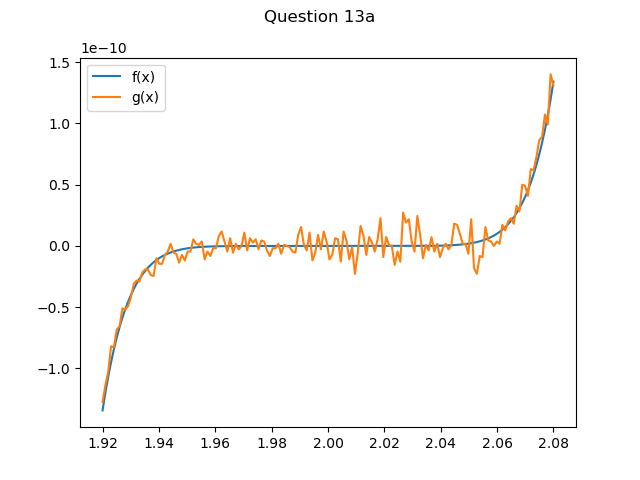
\includegraphics[width=.5\textwidth]{"../python/question13.png"}
    \end{center}
    \item
    Draw your conclusion from your results of Part (c) in Prob. 11 and Parts (a) and (b) in this problem.

    The plot shown very clearly demonstrates the stability of using $f(x)$ rather than $g(x)$ for numerics. It can be easily seen that $g(x)$ becomes very ragged when near $x = 2$ which $f(x)$ does not demonstrate at all. This is perhaps from numerical errors in the large amplitude of the terms in $g(x)$ as opposed to the single term in $f(x)$. 
   \end{enumerate}
    


\end{enumerate}




\end{document}
